\chapter{Result}

%My hypothesis before start

\section{Sample data from Survey}

Independence of observations. This is mostly a study design issue and, as such, you will need to determine whether you believe it is possible that your observations are not independent based on your study design (e.g., group work/families/etc). A lack of independence of cases has been stated as the most serious assumption to fail. Often, there is little you can do that offers a good solution to this problem. %https://statistics.laerd.com/statistical-guides/one-way-anova-statistical-guide-2.php

%Indepencence: Chi-square Test of Independence -  researching if two categorical variables are related or associated (i.e. dependent).  https://onlinecourses.science.psu.edu/stat500/node/56

Designed the survey so that the observations should be random and independent \\
- Random order on the tests \\
- Random color on the layers \\
- Random which order the layers was drawn on the map \\
- Random which order the metadata was written in the table \\

\section{Statistics theory}
This section will give an introduction to the statistics used in this thesis. The thesis will examine the data with parametric methods but also with non-parametric methods if the assumption of a normally distributed samples fails. A nonparametric method is much more efficient than the parametric procedure when the set of data used in the test deviates significantly from the normal distribution \citep{Walpole2012}. There are also some disadvantages using nonparametric methods. The methods will be less efficient, and to acchieve the same power as the corresponding parametric method a larger sample size is required. If parametric and nonparametric tests are both valid on the same set of data, the parametric test should be used \citep{Walpole2012}. 

\subsection{Normal testing}\label{sec:normaltesting}
The sampling distribution of a statistic depend on the distribution of the population, the size of the samples, and the method of choosing the samples \citep{Walpole2012}. Sampling distibution describes the variability of sample averages around the population mean $\mu$. All parametric statistics assumes normally distributed, independent observations. Parametric tests are preffered in statistics because it got more statistical power than nonparametric tests \citep{Frost2015}. The power of a test is the probability of correctly rejecting a false null hypothesis, which in this case is the ability to detect if the sample comes from a non-normal distribution. To determine if a sample is normally distrubuted there exists both visual methods and normality tests to assess the samples normality. A visual inspection of the sample's distribution is usually unreliable and does not guarantee that the distribution is normal \citep{Pearson2006}. Presenting the data visually gives the reader an opportunity to judge the distribution themselves. In this thesis histograms are used to visualize the data for normality. 

Normality tests compare the scores in the sample to a normally distributed set of scores with the same mean and standard deviation \citep{Ghasemi2012}. There are multiple normality tests, and deciding which test to use is not easy. This study needs a test that doesn't require every value to be unique, a test that can handle ties (identical observations). The survey used to collect the samples in this study do not guarantee unique values. 

The D'Agostino-Pearson omnibus test stand out as the best choice. This test first computes the skewness, see figure \ref{fig:skew}, and kurtois, see figure \ref{fig:kurtois}, to quantify how far from the normal distribution the sample is from the terms of assymetry and shape. Then it calculates how far each of these values differs from the value expected with a normal distribution \citep{Pearson2006}. It works well even if all values are not unique \citep{Motulsky2013}. The test also works well on both short- and long-tailed distributions \citep{Yap2011}. \newline  %THIS STUDY HAS?? LONG OR SHORT??

\begin{figure}[h!]
	\centering
	\includegraphics[width=0.7\linewidth]{"fig/skew"}
	\caption{Skew \citep{MedCalcSoftwarebvba2017}}
	\label{fig:skew}
\end{figure}

\begin{figure}[h!]
	\centering
	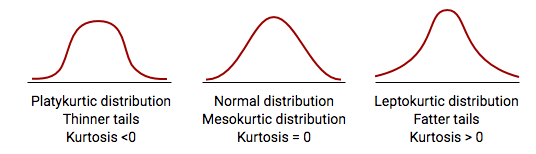
\includegraphics[width=0.7\linewidth]{fig/kurtois}
	\caption{Kurtois \citep{MedCalcSoftwarebvba2017}}
	\label{fig:kurtois}
\end{figure}


The D'Agostino-Pearson test uses the following hypothesis:\newline

\centerline{$H_{0}$: The data follows the normal distribution} 
\centerline{$H_{A}$: The data do not follow the normal distribution}

For small sample sizes, normality tests have little power to reject the null hypothesis, therefore small sample sizes most often pass normality tests. For large sample sizes, significant results would be derived even in the case of a small deviation from normality \citep{Pearson2006}. When the null hypothesis cannot be rejected, then there are two possible cases. First case is to accept the null hypothesis or the second case is that the sample size is not large enough to either accept or reject the null hypothesis \citep{ThePennsylvaniaStateUniversity2017}. An acceptance of the null hypothesis implies that the evidence was insufficient, the result does not necessary accept $H_{0}$, but fails to reject $H_{0}$ \citep{Walpole2012}.  

%A \textit{goodness-of-fit} test is used to determine whether a sample of \textit{n} observations can be considered as a sample from a given specified distribution \citep{Walpole2012}. The Anderson-Darling and the Kolmogorov-Smirow tests stand out as \textit{goodness-of-fit} procedures specialized for small samples \citep{Romeu2003}. The Anderson-Darling test will be used in this study to test if the observations gathered in this study is normally distributed.  %The Kolmogorov-Smirow test is a nonparametric test. The hypothesis for the Anderson-Darling test is: \newline

%\centerline{$H_{0}$: The data follows the normal distribution} 
%\centerline{$H_{A}$: The data do not follow the normal distribution}

%The computations in the Anderson-Darling test differs based on what is known about the observations. In this study both the expected mean and variance is unknown. In all the Anderson-Darling tests in this study a significance level of $0.05$ is used, which gives a confidence interval of $95$ \% . If the calculated \textit{p-value} is less than the significance level ($0.05$), the null hypothesis is rejected. The larger the \textit{p-value} the closer match is the data to the normal distribution. The Anderson-Darling statistics is used to calculate the \textit{p+value} for the \textit{goodness-of-fit} test. 
\subsection{Bionomal disstibution}
Used for discrete variables. It used the probability of getting $x$ successes and $n-x$ failures in $n$ trials. Each success comes with a probability $p$ and each failure with probability $q=1-p$  [\citep{Walpole2012}, p. 145]. The sample mean $\overline{x}$ and variance of $\overline{x}$ of the bionomial distribution is: $\overline{x} = n * p$ and $\sigma^{2} = n*p*q$. The probability p has to be the same on every trial - NOT TRUE HERE.

In the survey, the number of correctly chosen elements is recorded. Here x = the number of correct elements. x is a random variable who has the binomial distribution. The following null and alternative hypothesis can be used:

\centerline{$H_{0}$: All elements are correctly chosen in each task} 
\centerline{$H_{A}$: Not all element are correctly chosen in each task}

$p=\frac{\overline{x}}{n}$, if $p*n >= 5$ and $n*(1-p) > = 5$ then we can use the normal distribution. 

\subsection{Hypothesis testing}\label{sec:hypothesistesting}
The null- and alternative hypothesis are statements regarding a difference or an effect that occur in the population of the study. The alternative hypothesis (Ha) usually represents the question to be answered or the theory to be tested, while the null hypothesis ($H_{0}$) nullifies or opposes Ha \citep{Walpole2012}. The sample collected in the study is used to test which statement is most likely (technically it's testing the evidence against the null hypothesis).  When the hypothesis is identified, both null and alternative, the next step is to find evidence and develop a strategy for or against the null hypothesis \citep{LundResearchLtd2013}.

The first step, after identifying the hypothesis, is to determine the level of statistical significance, often expressed as the \textit{p-value}. A statistical test will result in the probability (\textit{the p-value}) of observing your sample results given that the null hypothesis is true. A significance level widely used in academic research is 0.05 or 0.01 \citep{Walpole2012}. 

You should not report the result as "significant difference", but instead report it as "statistically significant difference". This is because your decision as to whether the result is significant or not should not be based solely on your statistical test. Therefore, to indicate to readers that this "significance" is a statistical one, include this is your sentence \citep{LundResearchLtd2013a}. 

%Compare the mean time in experienced and not experienced
%H0: No time difference, Ha: Experienced use less time

\subsubsection{Two sample t-test}\label{sec:t-test}
When estimating the difference between two means a two-sample t-test is used \citep{Walpole2012}. A two sampled test assumes two independent, random samples from distributions with means [$\mu_{1}$ , $\mu_{2}$] and variances [$\sigma_{1}^{2}$, $\sigma_{2}^{2}$]. %*HOW TO DETERMINE IF THEY ARE INDEPENDENT? 
The hypothesis on two means can be written as:\newline

\centerline{$H_{0}$: $\mu_{1}$ - $\mu_{2}$ = 0 or $\mu_{1}$ = $\mu_{2}$} 
\centerline{$H_{A}$: $\mu_{1}$ - $\mu_{2}$ > 0 or $\mu_{1}$ > $\mu_{1}$}
 
Then the hypothesis refer to a one-tailed two sampled t-test. Before doing tests on the two means, the Levene's Test is used to test if the samples are from populations with equal variances. It tests the hypothesis:\newline %https://docs.scipy.org/doc/scipy-0.14.0/reference/generated/scipy.stats.levene.html

\centerline{$H_{0}$: Input samples are from populations with equal variances} 
\centerline{$H_{A}$: Input samples are from populations that do not have equal variances}

If we can assume equal variances in the two samples and the samples are normal distributed, a two-sampled t-test may be used. 
%There are also formula for Unknown but unequal variances, page 345 in statistics book

Because the one-sided tests can be backed out from the two-sided tests. (With symmetric distributions one-sided p-value is just half of the two-sided pvalue). It goes on to say that scipy always gives the test statistic as signed. This means that given p and t values from a two-tailed test, you would reject the null hypothesis of a greater-than test when p/2 < alpha and t > 0, and of a less-than test when p/2 < alpha and t < 0. %http://stackoverflow.com/questions/15984221/how-to-perform-two-sample-one-tailed-t-test-with-numpy-scipy
%https://docs.scipy.org/doc/scipy-0.18.1/reference/generated/scipy.stats.ttest_ind.html

Relevant hypothesis in this study that can be tested with a two-sampled t-test (if the conditions mentioned above are valid) is listed under. \newline

\begin{framed}{\noindent\centering
		
		\textit{Hypothesis - Two sample t-test} \newline
		
		\textbf{$H_{0}$:} Mean task time between participants are equal\\
		\textbf{$H_{A}$:} Experienced participants finish the tasks faster, use less time\newline
		
		$H_{0}$: Total number of correct elements between participants are equal \\
		$H_{A}$: Experienced participants have a higher number of correct elements\newline
		
		$H_{0}$: There are no difference in total number of correct elements between the tasks\\
		$H_{A}$: Participants have more correct elements on the one element task\newline
		
		$H_{0}$: There are no difference in mean time between the tasks\\    
		$H_{A}$: Participants finish the one element task faster  %* ONE element task or three??
		\par}
\end{framed}

Before solving the hypothesis the conditions needs to be testet. More on this later. %*WHICH SECTION?

\subsubsection[ANOVA]{Analysis-of-Variance}\label{sec:anova}
Analysis-of-Variance (\textit{ANOVA}) is according to \cite{Walpole2012} a very common procedure used for testing population means. Where a two sample t-test are restricted to consider no more than two population parameters, \textit{ANOVA} can test multiple population parameters. A part of the goal of \textit{ANOVA} is to determine if the differences among the means of two or more samples are what we would expect due to random variation alone, or due to variation beyond merely random effects. \textit{ANOVA} assumes normally distributed, independent, samples with equal variance. The equal variance assumtion will be tested with Levene's Test also mentioned in subsection \ref{sec:t-test}. 

One-way \textit{ANOVA} tests the null hypothesis that two or more groups have the same population mean given that the mean is measured on the same factor or variable in all groups\citep{LundResearchLtd2013a}. The hypothesis test can be written like this:\newline

\centerline{$H_{0}$:  $\mu_{1} =  \mu_{2} = ... = \mu_{k} $} 
\centerline{$H_{A}$:  At least two of the means are different}

$\mu$ equals the group mean and $k$ represents the number of groups. It is important to check that each group are normally distributed, not only the sample \citep{LundResearchLtd2013a}. The weakness of one-way \textit{ANOVA} is that it cannot tell which specific groups were significally different from each other if $H_{0}$ is rejected. To be able to determine which group a \textit{post hoc test} is used. 

In an one-way \textit{ANOVA} test there should be one variable and minimum three independent groups, which is an relevant approach considering the data produced from this thesis survey. There are at least two variables in the survey data, task time and number of correctly chosen elements. The survey result can be divided into three groups, one element task, three elements task and six elements task. Each entry in the sample should only be assigned to one group. Relevant hypothesis from the study that can be used in an one-way \textit{ANOVA} test is shown under. \newline

\begin{framed}
		\begin{center}
			\textit{Hypothesis - One-way \textit{ANOVA}} \newline
			
			$H_{0}$: Mean task time is not different between the three tasks\\
			$H_{A}$: Mean task time is different between at least two of the tasks\\
			\textit{Variable = time, group = tasks}\newline
			
			$H_{0}$: Total number of correct elements between the three tasks are equal \\
			$H_{A}$: Total number of correct elements between at least two of the tasks are not equal \\
			\textit{Variable = Number of correct elements, group = tasks}\newline
	\end{center}
\end{framed}

The hypothesis written above will be testen in the section blabla. %* Add correct section

%As regards the normality of group data, the one-way ANOVA can tolerate data that is non-normal (skewed or kurtotic distributions) with only a small effect on the Type I error rate. However, platykurtosis can have a profound effect when your group sizes are small. This leaves you with two options: (1) transform your data using various algorithms so that the shape of your distributions become normally distributed or (2) choose the nonparametric Kruskal-Wallis H Test which does not require the assumption of normality. https://statistics.laerd.com/statistical-guides/one-way-anova-statistical-guide-3.php

%The test can determine if the mean time (the variable) is significally different between the three tasks (the groups) given in the survey. It can also be used to determine if there are any significant different in mean time given the six different orders the task could serve in. A third test is to have number of correct elements as the variable and the three tasks as groups. More on this later. %*WHIch section?

\subsubsection[Wilcoxon]{Wilcoxon Rank-Sum test}\label{sec:Wilcoxon}
The Wilcoxon Rank-Sum test is an appropriate alternative to the two-sample t-test (see subsection \ref{sec:t-test}) when the normality assuptions do not hold, but the samples are still independend and have a continous distribution \citep{Walpole2012}. Since this method is nonparametric (or distribution-free) it do not require the assumption of normality. 

The hypothesis for Wilcoxon Rank-Sum Test is:\newline

\centerline{$H_{0}$:  $\tilde{\mu}_{1} =  \tilde{\mu}_{2} $} 
\centerline{$H_{A}$: $\tilde{\mu}_{1} >  \tilde{\mu}_{2} $ or $\tilde{\mu}_{1} <  \tilde{\mu}_{2} $ or $\tilde{\mu}_{1} \neq  \tilde{\mu}_{2} $}

The alternative hypothesis depends on what the test should determine. If the sample with mean $\tilde{\mu}_1$ is greater than, smaller than or unequal to the sample with mean $\tilde{\mu}_2$.  First select a random sample from each population with means $\tilde{\mu}_{1} $ and $ \tilde{\mu}_{2} $. If the sample sizes are different, let $n_{1}$ be the number of observations in the smallest sample and $n_{2}$ for the largest sample. Then $\tilde{\mu}_1$ will be the mean for the smallest sample. If there are ties (identical observations) in the sample a Mann-Whitey U test is preffered \citep{TheScipycommunity2017}. 

\subsubsection{Mann-Whitey U test}
Skriv om nødvendig, om vi bare bruker tid er det liten sannsynlighet at det et identiske målinger.. 

\subsubsection[Kruskal]{Kruskal-Wallis test}
The Kruskal-Wallis test is a nonparametric alternative to one-way \textit{ANOVA} (see subsection \ref{sec:anova})  \citep{Walpole2012}. This test should be used if the assumption of normal distribution failed. As mentioned in this sections introduction, a nonparametric method does not assume normality. This test is an generalization of the rank-sum test when there are more than 2 samples.

Kruskal-Wallis is used to test equality of means in one-way \textit{ANOVA}, so the hypothesis for the Kruskal-Wallis test is:\newline

\centerline{$H_{0}$:  $\mu_{1} =  \mu_{2} = ... = \mu_{k} $} 
\centerline{$H_{A}$: Minimum two of the $\mu_{k}$'s are different}

Here $\mu_{k}$ is the rank mean for the group k. As in Wilcoxon Rank-Sum test (subsection \ref{sec:Wilcoxon}), the number of observations in the smallest sample is assigned to $n_1$, the second smallest to $n_2$ and the largest sample is assigned to $n_k$. 

\section{Survey results}


- All participants ordered by age \\
- All participants ordered by age, excluded by task 4 \\
- All results in one task, ordered by age \\ 
- Average time per micro-task \\
- Is there a difference in task order number 1, 2, 3? time and correct \\
- Is there a difference in task number 1, 2, 3? time and correct  \\
Can use it to explain the data

\subsection{Gathered data}\label{sec:gathereddata}

The gathered data will be analyse on the two variables: 1) total time used to complete each task and 2) number of correctly chosen elements per task. Total time and number of correct elements adds time and correctly chosen elements on question one and question two together. Sample mean $\overline{x}$, standard deviation of $\overline{x}$, standard error ($\frac{standard deviation}{\sqrt{sample size}}$) of $\overline{x}$, minimum in sample and maximum in sample are listed in the tables. In these tables, results from the training task is removed. Only results from the three tasks is used. Maximum possible correct elements per task is twelve. There are six elements in question one and six elements in question two, and the number of correctly chosen elements in each task is added together, maximum twelve correctly chosen elements.

The tables in this section, (\ref{sec:gathereddata}), are task results from all participants and all three tasks, excluding the training task. Task results with total time longer than 2160 seconds are filtered out. This is to remove 4 outliers that spend more than twice the approximated time (average time on the survey was 1080 seconds in the pilot test). These 4 participants also answered that they were disturbed during the test.

 The samples are in the first subsection (\ref{sec:alltasks}) divided into experienced and inexperienced, but the three tasks are not separated in this sample. In subsection \ref{sec:taskdivided_all} the sample are separated into the three tasks, all participants are kept in the sample. Section \ref{sec:taskdivided_experienced}  and \ref{sec:taskdivided_inexperienced} separates the samples in the three tasks and also in experienced and inexperienced participants. 

\subsubsection{All,  experienced and inexperienced participants}\label{sec:alltasks}

The mean, standard deviation, minimum and maximum values are listen i table \ref{tab:totaltime_all} and \ref{tab:totalcorrect_all}. I. 

\begin{table}[H]
	\centering
	\begin{tabular}{l|l|l|l}
		Total time per task (seconds)   & All  & Experienced & Inexperienced \\ \hline
		Number of observations & 457    & 247      & 210   \\
		Sample mean $\overline{x}$     & 176.86 & 184.68     & 167.66      \\
		Standard deviation of $\overline{x}$  & 99.21  & 108.01  & 87.10   \\
		Standard error of $\overline{x}$  & 4.64  & 6.87  & 6.01  \\
		Minimum in sample & 26.00  & 44.00  & 26.00     \\
		Maximum in sample & 755.00 & 752.00    & 755.00    \\ \hline
	\end{tabular}
	\caption[All participants and all tasks]{Total time (\textit{4 entries per volunteer)}}
	\label{tab:totaltime_all}
\end{table}

\begin{figure}[H]
	\centering
	\begin{subfigure}[b]{0.32\textwidth}
		\centering
		\includegraphics[width=\linewidth]{../../thesis-statisticmethods/statistic_analysis/figures/all_participants/histogram/totaltime}
		\caption{All}
		\label{fig:totaltime_all}
	\end{subfigure}
	\begin{subfigure}[b]{0.32\textwidth}
		\centering
		\includegraphics[width=\linewidth]{../../thesis-statisticmethods/statistic_analysis/figures/experienced_participants/histogram/totaltime}
		\caption{Experienced}
		\label{fig:totaltime_experienced}
	\end{subfigure}
	\begin{subfigure}[b]{0.32\textwidth}
		\centering
		\includegraphics[width=\linewidth]{../../thesis-statisticmethods/statistic_analysis/figures/inexperienced_participants/histogram/totaltime}
		\caption{Inexperienced}
		\label{fig:totaltime_inexperienced}
	\end{subfigure}
	\caption[Total time, participants sorted]{Total time per task divided in  all-, experienced- and inexperienced-participants}
\end{figure}

\begin{table}[H]
	\centering
	\begin{tabular}{l|l|l|l}
		Correct elements per task  & All  & Experienced & Inexperienced \\ \hline
		Number of observations & 457    & 247  & 210   \\
		Sample mean $\overline{x}$   & 9.79 & 9.82  & 9.75  \\
		Standard deviation of $\overline{x}$   & 1.50  & 1.50  &  1.51 \\
		Standard error of $\overline{x}$   & 0.07  & 0.09 &  0.10 \\
		Minimum in sample & 4.00 & 5.00  &  4.00  \\
		Maximum in sample  & 12.00 & 12.00  & 12.00  \\ \hline
	\end{tabular}
	\caption[Correct elements, all participants and all tasks]{Number of correctly chosen elements (\textit{4 entries per volunteer)}}
	\label{tab:totalcorrect_all}
\end{table}

\begin{figure}[H]
	\centering
	\begin{subfigure}[b]{0.32\textwidth}
		\centering
		\includegraphics[width=\linewidth]{../../thesis-statisticmethods/statistic_analysis/figures/all_participants/histogram/total_correct_elements}
		\caption{All}
		\label{fig:totalcorrectelements_all}
	\end{subfigure}
	\begin{subfigure}[b]{0.32\textwidth}
		\centering
		\includegraphics[width=\linewidth]{../../thesis-statisticmethods/statistic_analysis/figures/experienced_participants/histogram/total_correct_elements}
		\caption{Experienced}
		\label{fig:totalcorrectelements_experienced}
	\end{subfigure}
	\begin{subfigure}[b]{0.32\textwidth}
		\centering
		\includegraphics[width=\linewidth]{../../thesis-statisticmethods/statistic_analysis/figures/inexperienced_participants/histogram/total_correct_elements}
		\caption{Inexperienced}
		\label{fig:totalcorrectelements_inexperienced}
	\end{subfigure}
	\caption[Correct elements, participants sorted]{Correctly chosen elements per task divided in  all-, experienced- and inexperienced-participants}
\end{figure}

\subsubsection{All participants, divided in task 1, task 2 and task 3}\label{sec:taskdivided_all}

In table \ref{tab:totaltime_tasks} and \ref{tab:totalcorrect_tasks} mean, standard deviation, minimum and maximum is listed for the three different task the participants did in the survey. Task 1 is the task that served the participants with one and one elements. Task 2 is the task that served the participants with three and three elements, and task 3 gave all six elements at the same time. 

\begin{table}[H]
	\centering
	\begin{tabular}{l|l|l|l}
		Total time per task (seconds) & One element task & Three elements task & Six elements task \\ \hline
		Number of observations & 152    & 153      & 152        \\
		Sample mean $\overline{x}$  & 174.44  &  174.55   &   181.60   \\
		Standard deviation of $\overline{x}$   & 101,23  & 94.72  & 102.00     \\
		Standard error of $\overline{x}$   & 8.21 & 7.66 & 8.27 \\
		Minimum in sample    & 47  & 26  &   38   \\
		Maximum in sample   & 657 & 755  & 752   \\ \hline
	\end{tabular}
	\caption[Total time, divided into task 1, 2 and 3]{Total time divided into task 1, task 2 and task 3}
	\label{tab:totaltime_tasks}
\end{table}

\begin{table}[H]
	\centering
	\begin{tabular}{l|l|l|l}
		Correct elements per task & One element task & Three elements task & Six elements task \\ \hline
		Number of observations & 152    & 153      & 152        \\
		Sample mean $\overline{x}$ & 10.13  &  9.67  &   9.55   \\
		Standard deviation of $\overline{x}$ & 1.40  & 1.54  & 1.50    \\
		Standard error of $\overline{x}$ & 0.11 &  0.12 & 0.12  \\
		Minimum in sample  & 5.00  & 5.00  &   4.00  \\
		Maximum in sample  & 12.00 & 12.00  & 12.00 \\ \hline
	\end{tabular}
	\caption[Correct elements, divided into task 1, task 2 and task 3]{Number of correctly chosen elements divided into task 1, task 2 and task 3}
	\label{tab:totalcorrect_tasks}
\end{table}

\subsubsection{Experienced participants, divided in task 1, task 2 and task 3}\label{sec:taskdivided_experienced}

Dividing task 1, task 2 and task 3 results into experienced and inexperienced. Table \ref{tab:totaltime_tasks_experienced} are data gathered about experienced participants total time per task. Table \ref{tab:totalcorrect_tasks_experienced} are data gathered about experienced participants number of correctly chosen elements per task.

\begin{table}[H]
	\centering
	\begin{tabular}{l|l|l|l}
		Total time per task & One element task & Three elements task & Six elements task \\ \hline
		Number of observations & 81    & 84      & 82   \\
		Sample mean $\overline{x}$  & 187.74  &  174.65  &  191.93   \\
		Standard deviation of $\overline{x}$ & 122.08  & 84.30  & 115.18    \\
		Standard error of $\overline{x}$ & 13.64  & 9.20 & 12.79   \\
		Minimum in sample   & 57.00  & 52.00 &  44.00  \\
		Maximum in sample  & 657.00 & 492.00  & 752.00 \\ \hline
	\end{tabular}
	\caption[Total time, task and experienved divided]{Experienced total time per task, divided by task}
	\label{tab:totaltime_tasks_experienced}
\end{table}

\begin{table}[H]
	\centering
	\begin{tabular}{l|l|l|l}
		Correct elements per task & One element task & Three elements task & Six elements task \\ \hline
		Number of observations & 81    & 84      & 82   \\
		Sample mean $\overline{x}$ & 10.23  &  9.69  &  9.51   \\
		Standard deviation of $\overline{x}$ & 1.30  & 1.62  & 1.46   \\
		Standard error of $\overline{x}$ & 0.14  & 0.18  & 0.16   \\
		Minimum in sample & 7.00 & 5.00 &  5.00 \\
		Maximum in sample  & 12.00 & 12.00  & 12.00 \\ \hline
	\end{tabular}
	\caption[Correct elements, task and experienved divided]{Experienced participant's number of correct elements per task, divided by task}
	\label{tab:totalcorrect_tasks_experienced}
\end{table}

\subsubsection{Inexperienced participants, divided in task 1, task 2 and task 3}\label{sec:taskdivided_inexperienced}

Table \ref{tab:totaltime_tasks_inexperienced} are mean time, standard deviation, minimum time and maximum time spent on each task for inexperienced participants. Number of correctly chosen elements per task for inexperienced participants is shown in table \ref{tab:totalcorrect_tasks_inexperienced}. 

\begin{table}[H]
	\centering
	\begin{tabular}{l|l|l|l}
		Total time per task (seconds) & One element task & Three elements task & Six elements task \\ \hline
		Number of observations & 71    & 69  & 70   \\
		Sample mean $\overline{x}$  & 159.28  &  174.42  &  169.50  \\
		Standard deviation of $\overline{x}$  & 68.24  & 106.69  & 83.17   \\
		Standard error of $\overline{x}$  & 8.10  & 12.84  & 9.94   \\
		Minimum in sample & 47.00 & 26.00 &  38.00 \\
		Maximum in sample & 487.00 & 755.00  & 529.00  \\ \hline
	\end{tabular}
	\caption[Total time, inexperienced per task]{Inexperienced participant's time spent per task, divided by task}
	\label{tab:totaltime_tasks_inexperienced}
\end{table}

\begin{table}[H]
	\centering
	\begin{tabular}{l|l|l|l}
		Correct elements per task & One element task & Three elements task & Six elements task \\ \hline
		Number of observations & 71    & 69  & 70  \\
		Sample mean $\overline{x}$  & 9.99  &  9.65  &  9.60  \\
		Standard deviation of $\overline{x}$  & 1.50  & 1.45  & 1.56   \\
		Standard error of $\overline{x}$  & 0.18 & 0.17 & 0.19  \\
		Minimum in sample  & 5.00 & 6.00 &  4.00  \\
		Maximum in sample  & 12.00 & 12.00  & 12.00 \\ \hline
	\end{tabular}
	\caption[Correct elements, inexperienced per task]{Inexperienced participant's number of correct elements per task, divided by task}
	\label{tab:totalcorrect_tasks_inexperienced}
\end{table}

\subsection{Normality tests}
To check if a two-sample t-test (subsection \ref{sec:t-test}) and \textit{ANOVA}-test (subsection \ref{sec:anova}) can be used, the samples need to be tested if they are normally distributed or not. Both tests assumes normaly distributed samples. The normality section \ref{sec:normaltesting} concluded that the D'Agostino and Person normality test should be used in this thesis. A visual interpretation of histograms will also be a part of the normality tests. 

\subsubsection{Experienced and inexperienced participants}
The histograms \ref{fig:totaltimeexclude4_experienced} and \ref{fig:totaltimeexclude4_inexperienced} are positively skewed (see figure \ref{fig:skew}). This gives a strong evidence that the samples are not normally distributed. Samples involving time measurements are rarely normally distributed. This is because the sample will always be skewed since it is impossible to have negative time. There will always be a limit to how fast a participant can finish the tasks. 

\begin{figure}[H]
	\centering
	\includegraphics[width=0.7\linewidth]{../../thesis-statisticmethods/statistic_analysis/figures/experienced_participants/normalplot/totaltime_exclude4}
	\caption{Sample 1 - Experienced participants, total time}
	\label{fig:totaltimeexclude4_experienced}
\end{figure}

\begin{figure}[H]
	\centering
	\includegraphics[width=0.7\linewidth]{../../thesis-statisticmethods/statistic_analysis/figures/inexperienced_participants/normalplot/totaltime_exclude4}
	\caption{Sample 2 - Inexperienced participants, total time}
	\label{fig:totaltimeexclude4_inexperienced}
\end{figure}

An D'Agostino and Pearson normality test (\ref{sec:normaltesting}) confirmed the visual assessment conclusion with an significance level of 5\% (0.05). Both samples are not normally distributed with a confidence level of 95\%. 

\begin{tcolorbox}
		\begin{center}
			\textit{D'Agostino and Pearson normality test}\\
			Significance level: 95\%  \\[0.5cm]

			Sample 1: Experienced, total time per task\\
			P-value: $5.10 * 10^{-32}$\\
			P-value < 0.05 \\
			\underline{Sample 1 not normally distributed}	\\[0.5cm]
			
			Sample 2: Inexperienced, total time per task \\
			P-value: $3.34 * 10^{-32}$ \\
			P-value < 0.05 \\
			\underline{Sample 2 not normally distributed}	\\[0.5cm]
		\end{center}
\end{tcolorbox}

\cite{Osborne2010} claim that almost all analyses, even nonparametric tests, benefit from improving the normality of the samples, especially when the normality test is significantly denied. In both sample 1 and 2, the p-value was significantly lower than the significance level of 0.05. Data transformations are commonly used tools to improve normality of a sample distributions, but there are many types of data transformations. Common traditional transformations are square root or converting to logarithmic scales  \citep{Osborne2010}.    

%Boc-Cox Transformation? https://docs.scipy.org/doc/scipy-0.19.0/reference/generated/scipy.stats.boxcox.html https://www.isixsigma.com/tools-templates/normality/dealing-non-normal-data-strategies-and-tools/

%DIscrete variables http://stattrek.com/probability-distributions/discrete-continuous.aspx
